\documentclass{standalone}
\usepackage{tikz}
\usetikzlibrary{patterns, positioning}
\usepackage[sfdefault]{ClearSans} %% option 'sfdefault' activates Clear Sans as the default text font
\usepackage[T1]{fontenc}

\begin{document}
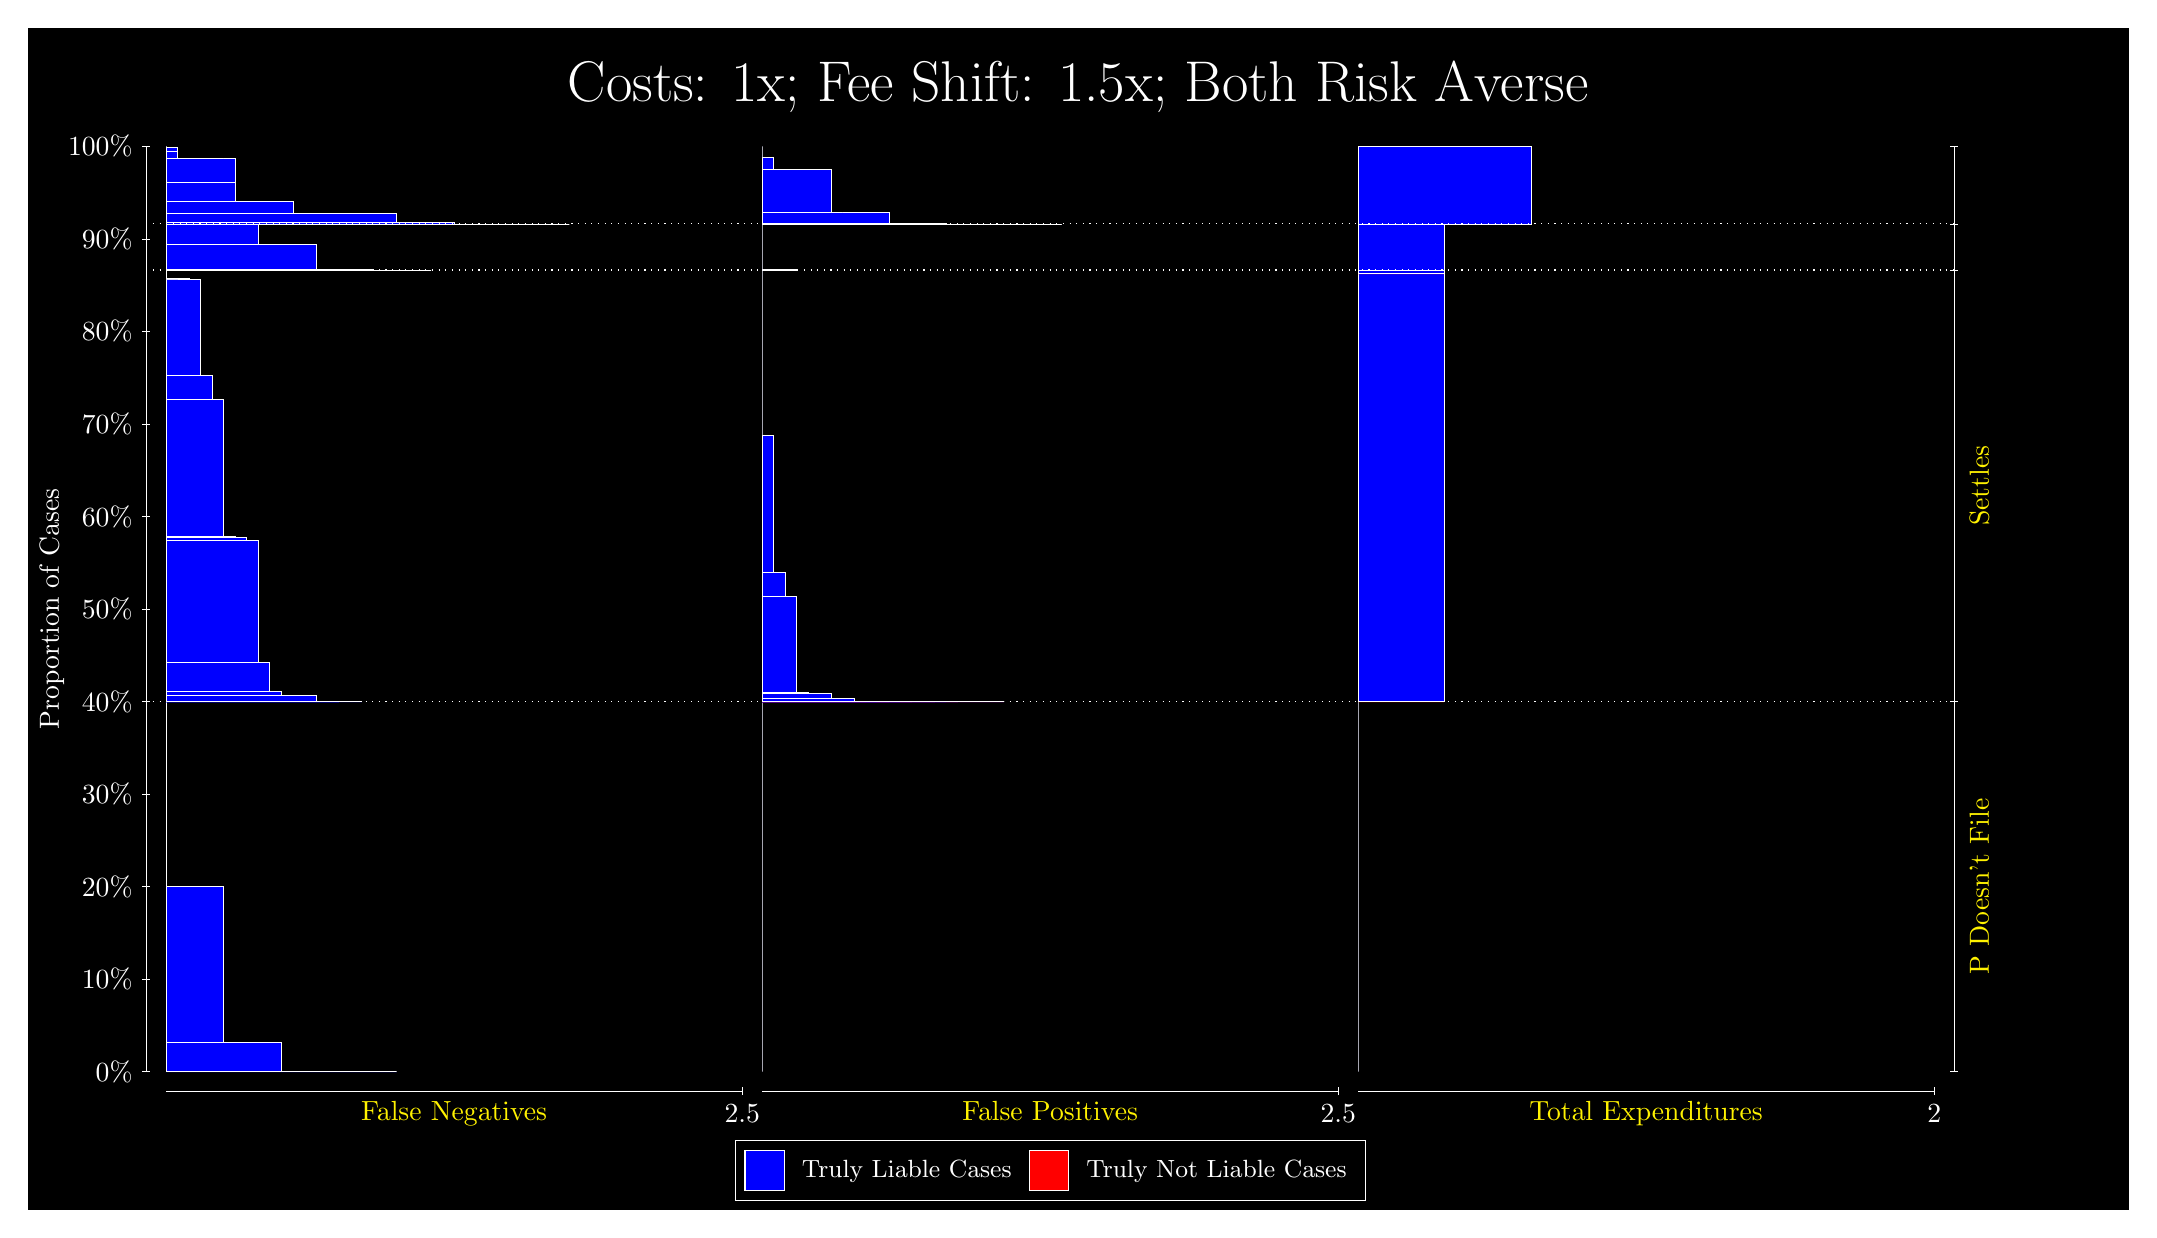
\begin{tikzpicture}
\draw[fill=black] (0,0) rectangle (26.667,15);
\draw[text=white] (0,13.5) rectangle (26.667,15) node[midway] {\huge Costs: 1x; Fee Shift: 1.5x; Both Risk Averse};
\draw[white, very thin] (1.5,1.75) -- (1.5,13.5);
\node[rotate=90, text=white, anchor=center] at (0.3, 7.625) {Proportion of Cases};
\draw[white, very thin] (1.45,1.75) -- (1.55,1.75);
\node[text=white, anchor=east] at (1.45, 1.75) {0\%};
\draw[white, very thin] (1.45,2.925) -- (1.55,2.925);
\node[text=white, anchor=east] at (1.45, 2.925) {10\%};
\draw[white, very thin] (1.45,4.1) -- (1.55,4.1);
\node[text=white, anchor=east] at (1.45, 4.1) {20\%};
\draw[white, very thin] (1.45,5.275) -- (1.55,5.275);
\node[text=white, anchor=east] at (1.45, 5.275) {30\%};
\draw[white, very thin] (1.45,6.45) -- (1.55,6.45);
\node[text=white, anchor=east] at (1.45, 6.45) {40\%};
\draw[white, very thin] (1.45,7.625) -- (1.55,7.625);
\node[text=white, anchor=east] at (1.45, 7.625) {50\%};
\draw[white, very thin] (1.45,8.8) -- (1.55,8.8);
\node[text=white, anchor=east] at (1.45, 8.8) {60\%};
\draw[white, very thin] (1.45,9.975) -- (1.55,9.975);
\node[text=white, anchor=east] at (1.45, 9.975) {70\%};
\draw[white, very thin] (1.45,11.15) -- (1.55,11.15);
\node[text=white, anchor=east] at (1.45, 11.15) {80\%};
\draw[white, very thin] (1.45,12.325) -- (1.55,12.325);
\node[text=white, anchor=east] at (1.45, 12.325) {90\%};
\draw[white, very thin] (1.45,13.5) -- (1.55,13.5);
\node[text=white, anchor=east] at (1.45, 13.5) {100\%};

\draw[white, very thin] (24.457,1.75) -- (24.457,13.5);
\draw[white, very thin] (24.407,1.75) -- (24.507,1.75);
\node[anchor=west] at (24.407, 1.75) {};
\draw[white, very thin] (24.407,6.4489) -- (24.507,6.4489);
\node[anchor=west] at (24.407, 6.4489) {};
\draw[white, very thin] (24.407,11.93) -- (24.507,11.93);
\node[anchor=west] at (24.407, 11.93) {};
\draw[white, very thin] (24.407,12.515) -- (24.507,12.515);
\node[anchor=west] at (24.407, 12.515) {};
\draw[white, very thin] (24.407,13.5) -- (24.507,13.5);
\node[anchor=west] at (24.407, 13.5) {};

\draw[white, very thin, fill=blue] (1.75,1.75) rectangle (4.6775,1.75);
\draw[white, very thin, fill=blue] (1.75,1.75) rectangle (3.9457,1.7532);
\draw[white, very thin, fill=blue] (1.75,1.7532) rectangle (3.2138,2.126);
\draw[white, very thin, fill=blue] (1.75,2.126) rectangle (2.4819,4.1027);
\draw[white, very thin, fill=red] (1.75,4.1027) rectangle (1.75,4.1027);
\draw[white, very thin, fill=blue] (1.75,4.1027) rectangle (1.75,6.4489);
\draw[white, very thin, fill=blue] (1.75,6.4489) rectangle (4.2384,6.4489);
\draw[white, very thin, fill=blue] (1.75,6.4489) rectangle (3.9457,6.4491);
\draw[white, very thin, fill=blue] (1.75,6.4491) rectangle (3.6529,6.5324);
\draw[white, very thin, fill=blue] (1.75,6.5324) rectangle (3.5065,6.5341);
\draw[white, very thin, fill=blue] (1.75,6.5341) rectangle (3.3602,6.5346);
\draw[white, very thin, fill=blue] (1.75,6.5346) rectangle (3.2138,6.5849);
\draw[white, very thin, fill=blue] (1.75,6.5849) rectangle (3.0674,6.944);
\draw[white, very thin, fill=blue] (1.75,6.944) rectangle (2.921,8.5004);
\draw[white, very thin, fill=blue] (1.75,8.5004) rectangle (2.7746,8.5382);
\draw[white, very thin, fill=blue] (1.75,8.5382) rectangle (2.6283,8.5479);
\draw[white, very thin, fill=blue] (1.75,8.5479) rectangle (2.4819,10.287);
\draw[white, very thin, fill=blue] (1.75,10.287) rectangle (2.3355,10.589);
\draw[white, very thin, fill=blue] (1.75,10.589) rectangle (2.1891,11.813);
\draw[white, very thin, fill=blue] (1.75,11.813) rectangle (2.0428,11.82);
\draw[white, very thin, fill=blue] (1.75,11.82) rectangle (1.8964,11.82);
\draw[white, very thin, fill=red] (1.75,11.82) rectangle (1.75,11.82);
\draw[white, very thin, fill=blue] (1.75,11.82) rectangle (1.75,11.93);
\draw[white, very thin, fill=blue] (1.75,11.93) rectangle (5.1167,11.93);
\draw[white, very thin, fill=blue] (1.75,11.93) rectangle (4.3848,11.937);
\draw[white, very thin, fill=blue] (1.75,11.937) rectangle (3.6529,12.261);
\draw[white, very thin, fill=blue] (1.75,12.261) rectangle (2.921,12.512);
\draw[white, very thin, fill=blue] (1.75,12.512) rectangle (2.1891,12.515);
\draw[white, very thin, fill=red] (1.75,12.515) rectangle (1.75,12.515);
\draw[white, very thin, fill=blue] (1.75,12.515) rectangle (6.8732,12.515);
\draw[white, very thin, fill=blue] (1.75,12.515) rectangle (6.1413,12.515);
\draw[white, very thin, fill=blue] (1.75,12.515) rectangle (5.4094,12.539);
\draw[white, very thin, fill=blue] (1.75,12.539) rectangle (4.8239,12.539);
\draw[white, very thin, fill=blue] (1.75,12.539) rectangle (4.6775,12.648);
\draw[white, very thin, fill=blue] (1.75,12.648) rectangle (4.092,12.648);
\draw[white, very thin, fill=blue] (1.75,12.648) rectangle (3.9457,12.654);
\draw[white, very thin, fill=blue] (1.75,12.654) rectangle (3.3602,12.801);
\draw[white, very thin, fill=blue] (1.75,12.801) rectangle (3.2138,12.801);
\draw[white, very thin, fill=blue] (1.75,12.801) rectangle (2.6283,13.039);
\draw[white, very thin, fill=blue] (1.75,13.039) rectangle (2.6283,13.348);
\draw[white, very thin, fill=blue] (1.75,13.348) rectangle (2.4819,13.348);
\draw[white, very thin, fill=blue] (1.75,13.348) rectangle (1.8964,13.433);
\draw[white, very thin, fill=blue] (1.75,13.433) rectangle (1.8964,13.494);
\draw[white, very thin, fill=red] (1.75,13.494) rectangle (1.75,13.494);
\draw[white, very thin, fill=blue] (1.75,13.494) rectangle (1.75,13.5);
\draw[white, very thin, fill=red] (9.3189,1.75) rectangle (9.3189,1.75);
\draw[white, very thin, fill=blue] (9.3189,1.75) rectangle (9.3189,6.4489);
\draw[white, very thin, fill=red] (9.3189,6.4489) rectangle (12.393,6.4489);
\draw[white, very thin, fill=blue] (9.3189,6.4489) rectangle (12.393,6.4489);
\draw[white, very thin, fill=red] (9.3189,6.4489) rectangle (11.807,6.4489);
\draw[white, very thin, fill=blue] (9.3189,6.4489) rectangle (11.807,6.4489);
\draw[white, very thin, fill=blue] (9.3189,6.4489) rectangle (11.661,6.4489);
\draw[white, very thin, fill=red] (9.3189,6.4489) rectangle (11.515,6.4489);
\draw[white, very thin, fill=blue] (9.3189,6.4489) rectangle (11.515,6.4489);
\draw[white, very thin, fill=red] (9.3189,6.4489) rectangle (11.222,6.4489);
\draw[white, very thin, fill=blue] (9.3189,6.4489) rectangle (11.222,6.4489);
\draw[white, very thin, fill=blue] (9.3189,6.4489) rectangle (11.075,6.4489);
\draw[white, very thin, fill=red] (9.3189,6.4489) rectangle (10.929,6.4489);
\draw[white, very thin, fill=blue] (9.3189,6.4489) rectangle (10.929,6.449);
\draw[white, very thin, fill=blue] (9.3189,6.449) rectangle (10.783,6.449);
\draw[white, very thin, fill=red] (9.3189,6.449) rectangle (10.636,6.449);
\draw[white, very thin, fill=blue] (9.3189,6.449) rectangle (10.636,6.449);
\draw[white, very thin, fill=blue] (9.3189,6.449) rectangle (10.49,6.4896);
\draw[white, very thin, fill=blue] (9.3189,6.4896) rectangle (10.344,6.4919);
\draw[white, very thin, fill=blue] (9.3189,6.4919) rectangle (10.197,6.5583);
\draw[white, very thin, fill=blue] (9.3189,6.5583) rectangle (10.051,6.5587);
\draw[white, very thin, fill=blue] (9.3189,6.5587) rectangle (9.9044,6.5657);
\draw[white, very thin, fill=blue] (9.3189,6.5657) rectangle (9.758,7.7895);
\draw[white, very thin, fill=blue] (9.3189,7.7895) rectangle (9.6116,8.0911);
\draw[white, very thin, fill=blue] (9.3189,8.0911) rectangle (9.4652,9.8306);
\draw[white, very thin, fill=blue] (9.3189,9.8306) rectangle (9.3189,11.93);
\draw[white, very thin, fill=red] (9.3189,11.93) rectangle (9.758,11.93);
\draw[white, very thin, fill=blue] (9.3189,11.93) rectangle (9.758,11.933);
\draw[white, very thin, fill=blue] (9.3189,11.933) rectangle (9.3189,12.515);
\draw[white, very thin, fill=red] (9.3189,12.515) rectangle (13.125,12.515);
\draw[white, very thin, fill=blue] (9.3189,12.515) rectangle (13.125,12.515);
\draw[white, very thin, fill=red] (9.3189,12.515) rectangle (12.393,12.515);
\draw[white, very thin, fill=blue] (9.3189,12.515) rectangle (12.393,12.515);
\draw[white, very thin, fill=red] (9.3189,12.515) rectangle (11.661,12.515);
\draw[white, very thin, fill=blue] (9.3189,12.515) rectangle (11.661,12.521);
\draw[white, very thin, fill=red] (9.3189,12.521) rectangle (10.929,12.521);
\draw[white, very thin, fill=blue] (9.3189,12.521) rectangle (10.929,12.667);
\draw[white, very thin, fill=red] (9.3189,12.667) rectangle (10.344,12.667);
\draw[white, very thin, fill=blue] (9.3189,12.667) rectangle (10.344,12.667);
\draw[white, very thin, fill=blue] (9.3189,12.667) rectangle (10.197,13.214);
\draw[white, very thin, fill=red] (9.3189,13.214) rectangle (9.6116,13.214);
\draw[white, very thin, fill=blue] (9.3189,13.214) rectangle (9.6116,13.214);
\draw[white, very thin, fill=blue] (9.3189,13.214) rectangle (9.4652,13.361);
\draw[white, very thin, fill=red] (9.3189,13.361) rectangle (9.3189,13.361);
\draw[white, very thin, fill=blue] (9.3189,13.361) rectangle (9.3189,13.5);
\draw[white, very thin, fill=red] (16.888,1.75) rectangle (16.888,1.75);
\draw[white, very thin, fill=blue] (16.888,1.75) rectangle (16.888,6.4489);
\draw[white, very thin, fill=red] (16.888,6.4489) rectangle (17.986,6.4489);
\draw[white, very thin, fill=blue] (16.888,6.4489) rectangle (17.986,11.883);
\draw[white, very thin, fill=red] (16.888,11.883) rectangle (17.986,11.883);
\draw[white, very thin, fill=blue] (16.888,11.883) rectangle (17.986,11.93);
\draw[white, very thin, fill=red] (16.888,11.93) rectangle (17.986,11.93);
\draw[white, very thin, fill=blue] (16.888,11.93) rectangle (17.986,12.515);
\draw[white, very thin, fill=red] (16.888,12.515) rectangle (19.083,12.515);
\draw[white, very thin, fill=blue] (16.888,12.515) rectangle (19.083,13.5);
\draw[white, dotted] (1.5,6.4489) -- (24.457,6.4489);
\draw[white, dotted] (1.5,11.93) -- (24.457,11.93);
\draw[white, dotted] (1.5,12.515) -- (24.457,12.515);
\draw[white, very thin] (1.75,1.5) -- (9.0689,1.5);
\node[text=yellow, anchor=north] at (5.4094, 1.5) {False Negatives};
\draw[white, very thin] (9.0689,1.45) -- (9.0689,1.55);
\node[text=white, anchor=north] at (9.0689, 1.45) {2.5};

\draw[white, very thin] (9.3189,1.5) -- (16.638,1.5);
\node[text=yellow, anchor=north] at (12.978, 1.5) {False Positives};
\draw[white, very thin] (16.638,1.45) -- (16.638,1.55);
\node[text=white, anchor=north] at (16.638, 1.45) {2.5};

\draw[white, very thin] (16.888,1.5) -- (24.207,1.5);
\node[text=yellow, anchor=north] at (20.547, 1.5) {Total Expenditures};
\draw[white, very thin] (24.207,1.45) -- (24.207,1.55);
\node[text=white, anchor=north] at (24.207, 1.45) {2};

\node[text=yellow, centered, rotate=90] at (24.777, 4.0995) {P Doesn't File};
\node[text=yellow, centered, rotate=90] at (24.777, 9.1893) {Settles};



\draw (12.978300999999998,1.5) node[draw=none] (baseCoordinate) {};
\begin{scope}[align=center]
        \matrix[scale=0.5, draw=white, below=0.5cm of baseCoordinate, nodes={draw}, column sep=0.1cm]{
            \node[rectangle, draw, minimum width=0.5cm, minimum height=0.5cm, fill=blue] {}; &
            \node[draw=none, font=\small, text=white] (B) {Truly Liable Cases}; &
            \node[rectangle, draw, minimum width=0.5cm, minimum height=0.5cm, fill=red] {}; &
            \node[draw=none, font=\small, text=white] (B) {Truly Not Liable Cases}; \\
            };
\end{scope}

\end{tikzpicture}
\end{document}